\chapter{Results and Future Work}\label{chapter:Conclusion}

\section{Numerical result validation}

The \texttt{AlgorithmAnalysis.jl} package has been tested across a range of first-order optimization algorithms over the $m$-strong $L$-smooth convex function class to verify its ability to automatically generate accurate worst-case performance guarantees. In the test cases presented in this section, performance guarantees produced by the package matches to the mathematically produced results in \cite{tutorial}, proving that the package successfully implement Lyapunov-based algorithm analysis.

For every plots in this section, we set the value of $m$ to 1 and sample 12 values of $L$ that are logarithmically spaced between 1 and 100, using a base-10 scale. This ensures uniform coverage across orders of magnitude, capturing both small and large condition numbers with equal density in log space. The convergence rate produced by the package is plotted it on the y-axis, while the x-axis plots the condition number $L/m$ of the tested $(m,L)$ values.

\subsection*{Gradient descent}

Continuing the example in Figure \ref*{ex_analysis}, we plot the package's derived worst-case convergence rate guarantee of the gradient descent algorithm with step size $\alpha = 2/(L+m)$ at optimizing 12 different $m$-strong $L$-smooth convex function classes, using the 12 sampled $L$ values. The plot of the result produced is presented in Figure \ref*{gd_results}.

\begin{figure}[h]
    \centering
    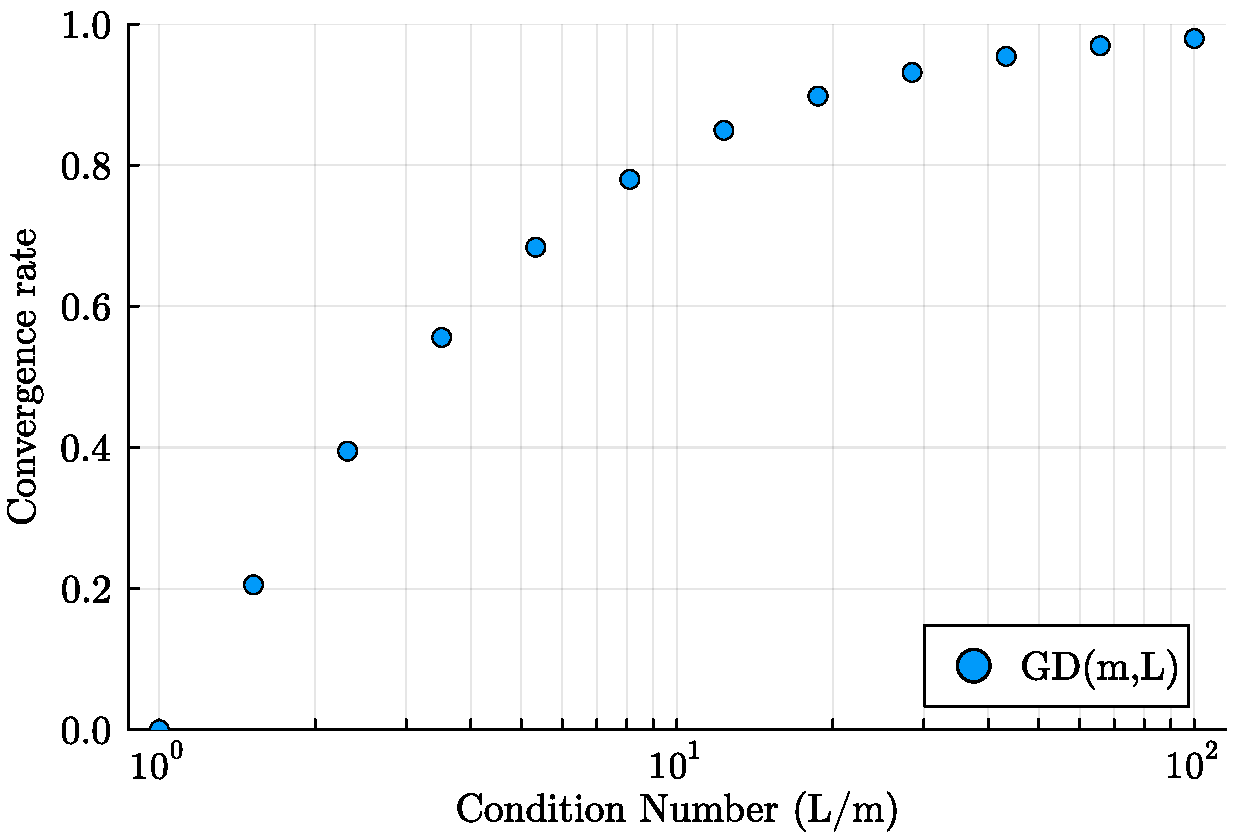
\includegraphics[width = .9 \textwidth]{gd_results.pdf}
    \caption{Convergence rate guarantee of gradient descent over sector smooth strongly convex classes}
    \label{gd_results}
\end{figure}

We have also tested the same gradient descent algorithm over 12 $(m, L)$ sector-bounded function classes. The code used to find the worst-case convergence rate guarantees of the fast gradient algorithm at optimizing $(m, L)$ sector-bounded function classes is presented in Figure \ref*{gd_sectorbounded_code} and the plot of the result produced is presented in Figure \ref*{gd_sectorbounded_results}. We expect the analysis result to be identical to that of gradient descent over $m$-strong $L$-smooth convex function classes.

\begin{figure}[h!]
	\begin{lstlisting}[mathescape]
$\alpha$ = 2/(L+m)
@algorithm begin
    f = DifferentiableFunctional{R$^n$}()
    xs = first_order_stationary_point(f)
    f' $\in$ SectorBounded(m, L, xs, f'(xs))
    x0 = R$^n$()
    x1 = x0 - $\alpha$*f'(x0)
    x0 => x1
    performance = (x0-xs)^2
end
@show rate(performance)
\end{lstlisting}
\caption{Analysis of GD and $m$-$L$ sector bounded functions}
\label{gd_sectorbounded_code}
\end{figure}

\begin{figure}[h]
    \centering
    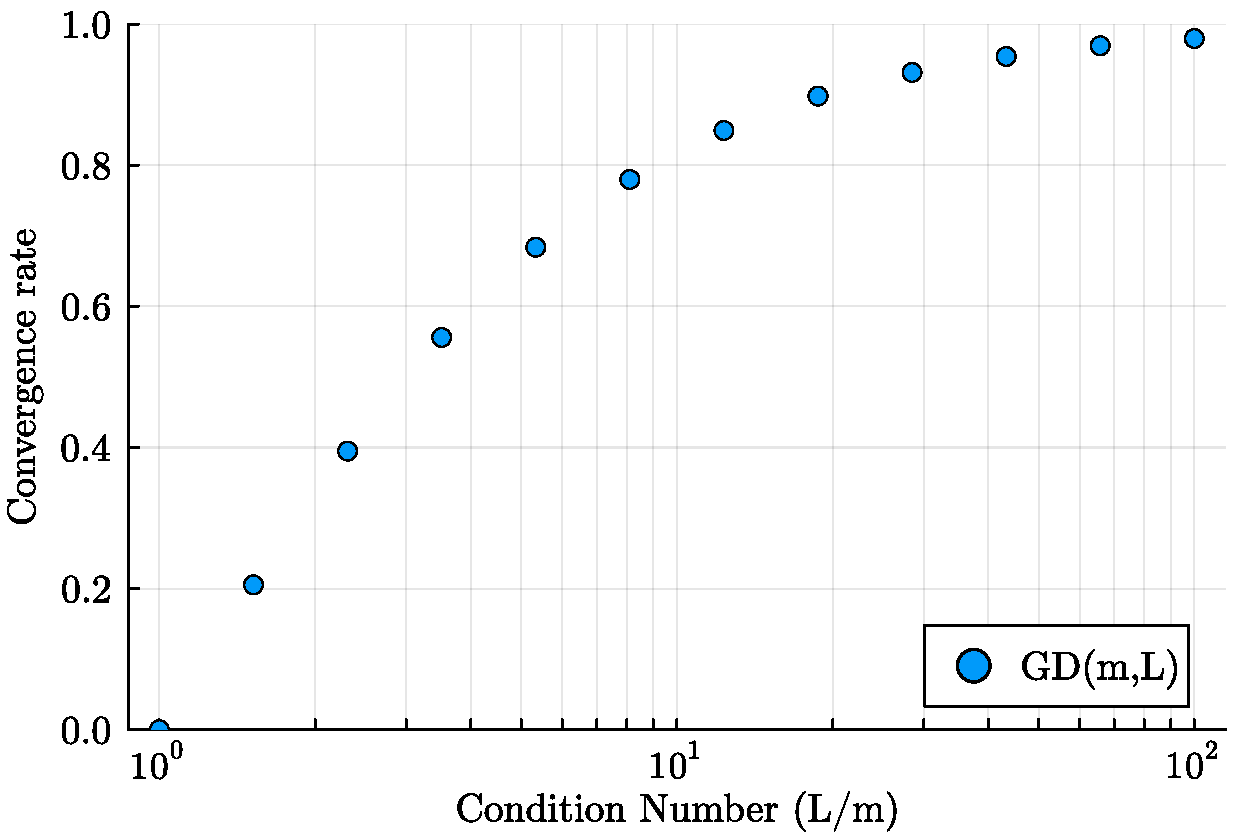
\includegraphics[width = .9 \textwidth]{gd_sectorbounded_results.pdf}
    \caption{Convergence rate guarantee of gradient descent over sector bounded function classes}
    \label{gd_sectorbounded_results}
\end{figure}
\subsection*{Fast gradient}

We tested the fast gradient algorithm with step sizes $\alpha = 4/(3L + m)$ and $\beta = (\sqrt{3L + 1} - 2)/(\sqrt{3L + 1} + 2)$. The code used to find the worst-case convergence rate guarantees of the fast gradient algorithm at optimizing $m$-strong $L$-smooth convex function classes is presented in Figure \ref*{fg_code} and the produced plot is presented in Figure \ref*{fg_results}.

\begin{figure}[h!]
	\begin{lstlisting}[mathescape]
$\alpha$ = 4/(3*L+m); $\beta$=(sqrt(3*L+1)-2)/(sqrt(3*L+1)+2)
@algorithm begin
    f = DifferentiableFunctional{R$^n$}()
    xs = first_order_stationary_point(f)
    f $\in$ SmoothStronglyConvex(m, L)
    x0 = R$^n$()
    x1 = R$^n$()
    y1 = x1 + $\beta$*(x1 - x0)
    x2 = y1 - $\alpha$*f'(y1)
    y2 = x2 + $\beta$*(x2 - x1)
    x3 = y2 - $\alpha$*f'(y2)
    x0 => x1
    x1 => x2
    x2 => x3
    performance = (y1-xs)^2
end
@show rate(performance)
\end{lstlisting}
\caption{Analysis of FG and $m$-smooth $L$-strongly convex functions}
\label{fg_code}
\end{figure}

\begin{figure}[h]
    \centering
    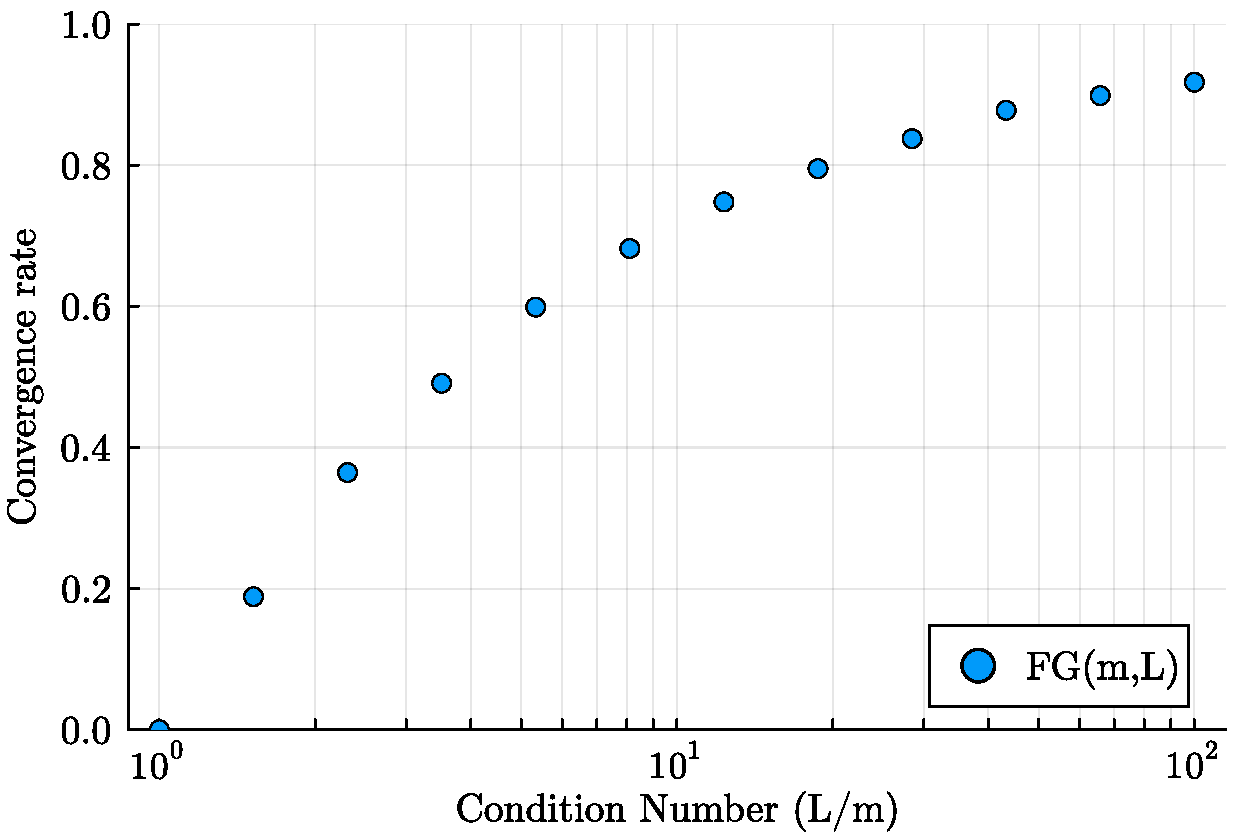
\includegraphics[width = .9 \textwidth]{fg_results.pdf}
    \caption{Convergence rate guarantee of fast gradient over smooth strongly convex function classes}
    \label{fg_results}
\end{figure}

\subsection*{Heavy ball}

We tested the heavy ball algorithm with the following step sizes:
\[
\alpha = \frac{4}{\left( \sqrt{L} + \sqrt{m} \right)^2}, \quad
\beta = \left( \frac{\sqrt{L/m} - 1}{\sqrt{L/m} + 1} \right)^2.
\]
The code used to find the worst-case convergence rate guarantees of the heavy ball algorithm for optimizing $m$-strongly convex and $L$-smooth function classes is presented in Figure~\ref{hb_code}, and the resulting plot is shown in Figure~\ref{hb_results}.


\begin{figure}[h!]
	\begin{lstlisting}[mathescape]
$\alpha$ = 4/((sqrt(L)+sqrt(m))^2); $\beta$=((sqrt(L/m)-1)/(sqrt(L/m)+1))^2
@algorithm begin
    f = DifferentiableFunctional{R$^n$}()
    xs = first_order_stationary_point(f)
    f $\in$ SmoothStronglyConvex(m, L)
    x0 = R$^n$()
    x1 = R$^n$()
    x2 = x1 - $\alpha$*f'(x1) + $\beta$*(x1-x0)
    x3 = x2 - $\alpha$*f'(x2) + $\beta$*(x2-x1)
    x0 => x1
    x1 => x2
    x2 => x3
    performance = (x0-xs)^2
end
@show rate(performance)
\end{lstlisting}
\caption{Analysis of HB and $m$-smooth $L$-strongly convex functions}
\label{hb_code}
\end{figure}

\begin{figure}[h]
    \centering
    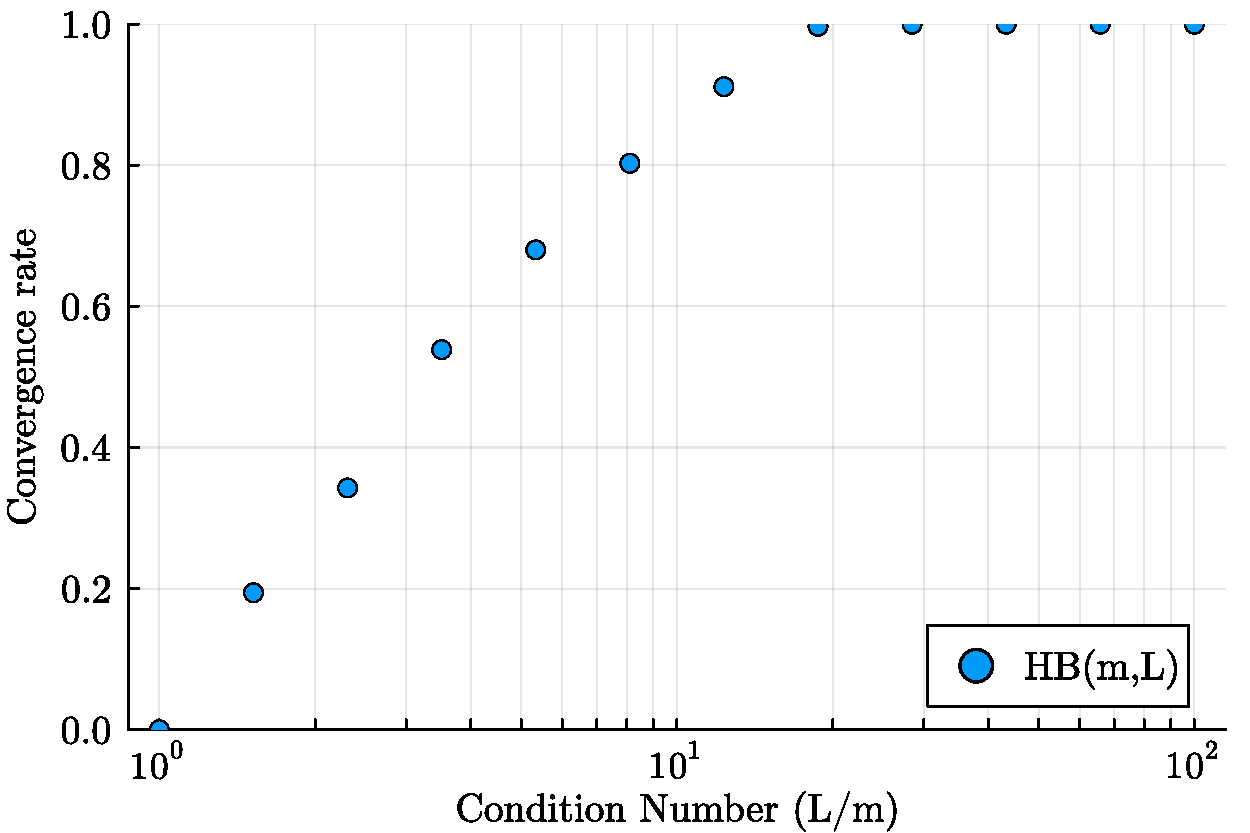
\includegraphics[width = .9 \textwidth]{hb_results.pdf}
    \caption{Convergence rate guarantee of heavy ball over smooth strongly convex function classes}
    \label{hb_results}
\end{figure}

\subsection*{Triple momentum}

We tested the triple momentum algorithm, which was developed by Van Scoy, Freeman, and Lynch in \cite{TMM} to be the fastest known globally convergent first-order algorithm at optimizing strongly convex functions. The algorithm is defined as:
\begin{equation}\label{eqn:GD}
    x_{k+1}= (1+\beta)x_{k} - \beta x_{k-1} - \alpha \nabla f((1+\gamma)x_k - \gamma x_{k-1})
  \end{equation}

The triple momentum algorithm's optimal parameters is determined by the condition number \( k = L/m \) when optimizing $m$-smooth $L$-strongly convex functions. The algorithm's parameters are defined as:

\[
\begin{aligned}
\rho &= 1 - \frac{1}{\sqrt{k}}, \\
\alpha &= \frac{1 + \rho}{L}, \\
\beta &= \frac{\rho^2}{2 - \rho}, \\
\gamma &= \frac{\rho^2}{(1 + \rho)(2 - \rho)}, \\
% \delta &= \frac{\rho^2}{1 - \rho^2}.
\end{aligned}
\]
Under these parameters, it was proven in \cite{TMM} that the performance guarantee matches the function $1-\sqrt{m/L}$, which is also plotted in along side the rates produced by the package in Figure~\ref{tmm_results}. The code used to find the worst-case convergence rate guarantees of the triple momentum algorithm is presented in Figure~\ref{tmm_code}.

\begin{figure}[h!]
    \centering
    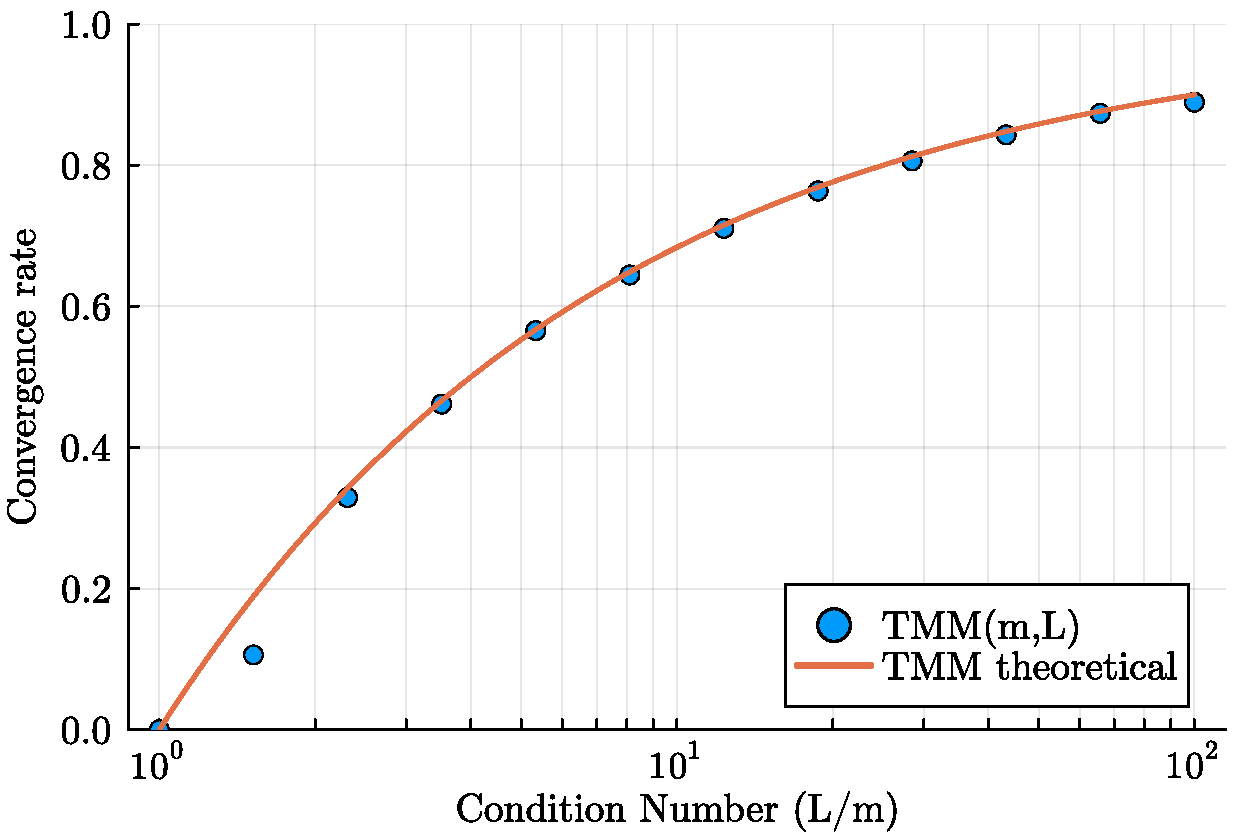
\includegraphics[width = .8 \textwidth]{tmm_results.pdf}
    \caption{Convergence rate guarantee of triple momentum over smooth strongly convex function classes}
    \label{hb_results}
\end{figure}

\begin{figure}[h!]
	\begin{lstlisting}[mathescape]
k = L/m
rho = 1 - 1/(sqrt(k))
$\alpha$ = (1 + rho)/L
$\beta$ = (rho^2)/(2-rho)
gamma = (rho^2)/((1+rho)*(2-rho))
delta = (rho^2)/(1-rho^2)
@algorithm begin
    f = DifferentiableFunctional{R$^n$}()
    xs = first_order_stationary_point(f)
    f $\in$ SmoothStronglyConvex(m, L)
    x0 = R$^n$()
    x1 = R$^n$()
    y1 = (1+gamma)*x1 - gamma*x0
    x2 = (1+$\beta$)*x1 - $\beta$*x0 - $\alpha$*f'(y1)
    y2 = (1+gamma)*x2 - gamma*x1
    x3 = (1+$\beta$)*x2 - $\beta$*x1 - $\alpha$*f'(y2)
    x0 => x1
    x1 => x2
    x2 => x3
    performance = ((1+delta)*x2 - delta*x1 -xs)^2
    
@show rate(performance)
\end{lstlisting}
\caption{Analysis of HB and $m$-smooth $L$-strongly convex functions}
\label{tmm_code}
\end{figure}

\section{Future work}

While the current experimental validations demonstrate that the \texttt{AlgorithmAnalysis.jl} package accurately generates worst-case performance guarantees for several prominent first-order optimization methods, we can explore other other methods to test compatibility. Future work should focus on systematically testing and verifying the package against a wider range of first-order unconstrained optimization algorithms. This extended analysis will further confirm the robustness of the package's implementation of the Lyapunov fucntion-based approach and highlight any potential limitations to be remedied and improved.

Additionally, the program currently does not support automatic ''lifting dimension'', a step of the Lyapunov method to algorithm analysis in \cite{tutorial}. While the user can manually add a lifting dimension by defining the analyze algorithm using more updates than the required 2. A function which can create these extra updated states, label them, and add them to the analysis process can allow the user to implement lifting dimension having only to enter how many extra updated states they wish to use. The lifting dimension will increase the size of the Lyapunov functions and introduce additional interpolated points and therefore additional constraints. As a result, the optimization problem we are solving to certify a convergence rate will becore more complexto the optimization problem while this research work is to implement this step and measure its effect on the tightness of the convergence rate guarantee.

